% Below is your UAH LaTeX template. This is the main fail that compiles your document. You will need to fill out the appropriate sections below. 

\documentclass[oneside, 12pt]{book} % Document class


\usepackage[utf8]{inputenc} % Basic package for Latex
\usepackage{graphicx} % To help include figures
\usepackage{geometry} % To allow document margin changes
\usepackage{setspace} % To allow custom spacing 
\usepackage{indentfirst} % To allow indentations in the first paragraph.
\usepackage{amsmath} % For formatting equations properly
\usepackage{natbib} % For formatting the bibliography
\usepackage{chngcntr} % To allow changing how figures, tables, and pages are counted.
\usepackage{appendix} % To help format the appendix
\usepackage[font=small,labelfont=bf]{caption} %This makes caption font small and makes the caption heading bold.
\usepackage{tabularx} %To allow formatting Tables.
\usepackage{array} %To allow creating arrays. 
\providecommand\phantomsection{} %This command allows you to make phantom sections that have no title but are still included in the Table of Contents such as the epigraph.
\usepackage[all]{nowidow} %This prevents widow/orphan lines
\usepackage{tikz}%This package helps to anchor the seal on the title page to the student name
\usetikzlibrary{tikzmark}%This is part of the tikz package


%Creating an Interlude Environment in order to NOT count or number a certain page such as the copyright page.
\newenvironment{interlude}{
  \clearpage
  \thispagestyle{empty}% we want this page to be empty (adjust to use a modified page style)
  \pagestyle{empty}% use the same style for subsequent pages in the unnumbered section
  }
  {\clearpage}

%The following package and lines can be used to format and create a list of symbols, equations, abbreviations, etc. The example actually used in this template is the \glossaries package, but you may also use this \nomencl package if desired.
\usepackage[intoc]{nomencl}
\makenomenclature
\renewcommand{\nomname}{List of Symbols}

% This is to ensure the page numbers are centered and at the bottom.
\usepackage{fancyhdr}
\pagestyle{fancy}
\fancyhf{}
\renewcommand{\headrulewidth}{0pt}
\cfoot{\thepage}

%This defines a new page style for just the title page.
\fancypagestyle{logopage}{\fancyhf{}\renewcommand{\headrulewidth}{0pt}\fancyfoot[C]{\includegraphics[scale=0.3]{Figures/Color Grad Banner.png}}}

%this causes equations to be counted according to their chapter location
\counterwithin{equation}{chapter} %this causes equations to be counted according to their chapter location
\counterwithin{figure}{chapter}




%This formats the table of contents the way Dr. Hakkila wants it
\usepackage[titles]{tocloft}


%Removes the Duplicate Chapter
\setcounter{secnumdepth}{4}% Show down to subsubsection

\setlength{\cftchapindent}{-20pt}% Just some value...

\usepackage{xpatch}

\makeatletter
\xpatchcmd{\@chapter}{\addcontentsline{toc}{chapter}{\protect\numberline{\thechapter}#1}}{%
                      \addcontentsline{toc}{chapter}{\protect\numberline{}#1}}{\typeout{Success}}{\typeout{Failed!}}
\makeatother



%This formats the Table of contents title
\renewcommand{\contentsname}{\hspace*{\fill}\bfseries\large Table of Contents\hspace*{\fill}}   


\renewcommand{\cftbeforetoctitleskip}{-0.25in}  

\renewcommand\cftchapdotsep{\cftdotsep}
\renewcommand\cftchapleader{\cftdotfill{\cftchapdotsep}}
%\renewcommand{\cftchappresnum}{CHAPTER } % put this before the number
%\addtolength{\cftchapnumwidth}{6em} % extra space for number and pre-name
%\renewcommand{\cftchapaftersnum}{. } % put period after chapter number and space


%This puts all the chapter headings into all-caps
%\renewcommand{\chaptername}{CHAPTER}

%Hopefully this reformats the List of Figures Title
\renewcommand{\listfigurename}{\hspace*{\fill}\bfseries\large List of Figures\hspace*{\fill}}  

%Reformat List of Tables, etc.
\renewcommand{\listtablename}{\hspace*{\fill}\bfseries\large List of Tables\hspace*{\fill}}  


%This creates a List of Equations.
\newcommand{\listequationsname}{List of Equations}
\newlistof{equations}{equ}{\listequationsname}

\newcommand{\eqdesc}[1]{%
  \csname phantomsection\endcsname % if hyperref is loaded
  \addcontentsline{equ}{equations}{\protect\numberline{\theequation}#1}%
}

\setlength{\parindent}{36pt}


%The following formats the chapter titles and sections appropriately
\usepackage{titlesec}



\titleformat
{\chapter}
[hang]
{\normalfont\large\bfseries\filcenter}
{} %Label. This is blank so that the entire chapter heading and title are properly centered. 
{0pt} %  Horizontal Space between label and title body.
{} %Before-Code 
{} 

\titleformat
{\section}
[hang]
{\normalfont\normalsize\bfseries}
{\thetitle} %Label. 
{.5em} %  Horizontal Space between label and title body.
{} %Before-Code 
{} 

\titleformat
{\subsection}
[hang]
{\normalfont\normalsize\bfseries}
{\thetitle} %Label. 
{.5em} %  Horizontal Space between label and title body.
{} %Before-Code 
{} 

\titlespacing{\subsection}{2em}{12pt}{12pt}

\titlespacing{\chapter}{0pt}{50pt}{12pt}

\titlespacing{\part}{0pt}{12pt}{12pt}


\titlespacing{name=\chapter, numberless}{0pt}{0pt}{12pt}


% I had used this code to combine the chapter heading and 
%\titleformat{\chapter}[hang] 
 % {\normalfont\large\bfseries\filcenter}{\chaptertitlename\ \thechapter:}{.3em}{} 


%This names the Bibliography/References whatever you want it to be.
\renewcommand{\bibname}{References}

%The below package creates the optional List of Symbols and formats it correction..
\usepackage[acronyms, automake, toc, nopostdot]{glossaries}
\usepackage{glossary-longbooktabs}
\newcolumntype{P}[1]{>{\centering\arraybackslash}p{#1}}
\renewcommand*{\entryname}{Symbol}
\newglossarystyle{mystyle}{% define custom glossaries style for Abbreviation page, read relative manual before change
\setglossarystyle{long-booktabs}%
\renewenvironment{theglossary}%
{\begin{longtable}{@{}P{3cm}@{}p{\dimexpr\linewidth-3cm}@{}}}%
{\end{longtable}}%

\renewcommand*{\glossaryheader}{%
 \bfseries\large Symbol & \centering\bfseries\large Description \tabularnewline\endhead \endfoot}%
}

\renewcommand{\glossarypreamble}{\normalsize}
\makeglossaries %To clean up this document, the preamble that includes the packages is located in the preamble.tex file found in the FrontMatter folder.

%********************************************
%********************************************
% THE SECTION BELOW MUST BE FILLED OUT 
%********************************************
%********************************************

%BASIC INFORMATION
\newcommand{\thesistitle}{Genomic changes associated with transitions to heterospory and genome downsizing in land plants.}
\newcommand{\studentname}{Rijan R. Dhakal}
\newcommand{\degree}{Master of Science in Biological sciences}%e.g., Master of Science in Engineering, Doctor of Philosophy, etc.
\newcommand{\department}{Biology}% Do not include the words "The department of." Just write the name of your department.
\newcommand{\gradyear}{2022}% complete 4 digit year, e.g., 2022
\newcommand{\gradmonth}{December}% Spell out the month completely, e.g., December
%\newcommand{\jointuni}{Auburn University} %If this is a joint degree, remove the % sign at the beginning of this line and enter the entire name of the additional universities.

%***********************
%SPECIFY THESIS OR DISSERTATION
% Below, if you are earning a master's degree, remove the "%" on the line below that says \newcommand{thesis}. If you are earning a PhD or other doctorate degree, remove the "%" on the line below that says \newcommand{dissertation}.

\newcommand{\thesis}{FOR MASTER'S STUDENTS ONLY}
%\newcommand{\dissertation}{FOR DOCTORATE DEGREE STUDENTS ONLY}

%*******************************
%SPECIFY THE PROFESSORS WHO WILL APPROVE YOUR THESIS/DISSERTATION
%Professor information: Fill out only their first and last name WITH NO PREFIXES OR SUFFIXES. If a line is not applicable, simply add a % sign at the beginning of that line. If there is an applicable line that has a % sign at the beginning, remove this sign and fill in as needed.
%\newcommand{\resadv}{Paul Wolf}
%\newcommand{\comchair}{Committee Chair Name}
\newcommand{\reschair}{Paul Wolf} %If your research advisor and committee chair are the same person, enter his/her name on this line.
\newcommand{\commema}{Paul Wolf}
\newcommand{\commemb}{Alex Harkess}
\newcommand{\commemc}{Jerome Baudry}
%\newcommand{\commemd}{[4th Committee Member Name]}
%\newcommand{\commeme}{[5th Committee Member Name]}
%\newcommand{\commemf}{[6th Committee Member Name]}
%\newcommand{\commemg}{[7th Committee Member Name]}
%\newcommand{\commemh}{[8th Committee Member Name]}
%\newcommand{\commemi}{[9th Committee Member Name]}
\newcommand{\depchair}{Paul Wolf}
\newcommand{\colldean}{Rainer Steinwandt}
\newcommand{\graddean}{Jon Hakkila}



%**************
%INDICATE IF YOU HAVE REGISTERED FOR A COPYRIGHT.
%**************
%\newcommand{\copyrightreg}{Yes} %If you registered for a copyright through Proquest, please remove the % sign from the beginning of this line starting with \newcommand{\copyrightreg}{Yes}. If you did not register for a copyright, no action is needed.  

%********************************************
%********************************************
% End of Section to Fill Out. 
%********************************************
%********************************************

\usepackage[colorlinks=true,linkcolor=black,anchorcolor=black,citecolor=black,filecolor=black,menucolor=black,runcolor=black,urlcolor=black]{hyperref} %This creates hyperlinks for chapter, figure, and table titles in your pdf. It should be the last package before the document begins.

%*********************************************
%*********************************************
%Optional List of Symbols/Abbreviations
%*********************************************
%*********************************************

%A list of symbols/abbreviations is optional. If you do not want to include one, simply delete this section from your document. You may also delete this section and use a different package as there are multiple packages that can be used to make a List of Symbols, Abbreviations, Nomenclature, Etc. Below uses the \glossaries-extra package. This package is nice if you want to include multiple lists or sections. The following links provide useful information on how to use this package.
% https://mirrors.mit.edu/CTAN/macros/latex/contrib/glossaries/glossariesbegin.pdf
% https://mirrors.rit.edu/CTAN/macros/latex/contrib/glossaries/glossaries-user.pdf
% https://www.overleaf.com/learn/latex/Glossaries


% This uses the glossaries package. With this package, you can include multiple types of lists, track page numbers if desired, and define new lists. More information can be found at the following sites: https://mirrors.mit.edu/CTAN/macros/latex/contrib/glossaries/glossariesbegin.pdf and https://mirrors.rit.edu/CTAN/macros/latex/contrib/glossaries/glossaries-user.pdf https://www.overleaf.com/learn/latex/Glossaries


%*****************************************
%Define your list of glossary items below. Remember that the entries that you enter in this file will not automatically appear in the List of Symbols. You also have to reference the symbol in the body of your thesis by using the \gls command. 

%symbols
\newglossaryentry{deg}{name=$^\circ$, description={Degree}}
\newglossaryentry{grav}{name={1D}, description={Normal gravity environment}}
\newglossaryentry{wf}{name={\textit{f}}, description={Wear factor}}
\newglossaryentry{alp}{name={$\alpha$},description={Alpha}}
\newglossaryentry{theta}{name={$r_O$}, description={ecosystem respiration at reference temperature $T_a=0{^\circ}$C}}
\newglossaryentry{te}{name={$\tau_e$}, description={precision of the normal distribution of the likelihood}}
\newglossaryentry{q10}{name={$Q_{10}$}, description={multiplication factor to respiration with 10$^\circ$C increases in $T_a$}}
\newglossaryentry{phi}{name={$\phi$}, description={vapour pressure deficit response function}}
\newglossaryentry{del}{name=$\delta$, description={Transition coefficient constant for the design of linear-phase FIR filters which are used to take up space when testing the list of symbols}}

 %Go to this page to enter all the symbols you plan to use in the document.

% Scroll down in this file to after the List of Tables section in order to actually add your Lists to your document,.

%**********************************************
%**********************************************
% End of Optional List of Symbols/Abbreviations
%**********************************************
%**********************************************



%******************************************
%******************************************
% Document Begins Here
%******************************************
%******************************************

\begin{document}

\frontmatter % This command creates the front matter environment.

%**********************************
%**********************************
%Title Page
%**********************************
%**********************************
% Do not directly edit this page. Everything on the Title Page should auto-fill if you correctly filled out the information on the main.tex file.

\begin{titlepage}
\newgeometry{left=1.5in,bottom=.5in}
    \begin{center}
        \large
        \singlespacing
        \textbf{\thesistitle}
        

\vspace{2cm}

        \Large
        \textbf{\studentname}\\
        \vspace{1.5cm}
        \normalsize
        \ifdefined\thesis
        \textbf{A THESIS}
        \vspace{1.5cm}
        \else
        \ifdefined\dissertation
        \textbf{A DISSERTATION}
        \vspace{1.5cm}
        \else
        Please identify this document as either a thesis or dissertation on the main.tex file in the section at the top that must be filled out.
        \vspace{1.5cm}
        \fi
        \fi

        \textbf{Submitted in partial fulfillment of the requirements \\for the degree of \degree}\\  
        
\vspace{0.1cm}
  \textbf{in}\\
      \vspace{0.1cm}
        \textbf{The Department of \department}\\
        \vspace{0.1cm}
  \textbf{to}\\
\vspace{0.1cm}
\textbf{The Graduate School}\\
\vspace{0.1cm}
\textbf{of}\\
\vspace{0.1cm}
        \ifdefined\jointuni
        \textbf{The University of Alabama in Huntsville\\ and\\  \jointuni}
        \else
        \textbf{The University of Alabama in Huntsville}
    \fi

        
        \vspace{0.4cm}
        \textbf{\gradmonth\ \gradyear}
        


    \end{center}
    

\vfill

\textbf{Approved by:}


\vspace{.1cm}
\setstretch{1.25}

\ifdefined\reschair
\noindent
Dr. \reschair, Research Advisor/Committee Chair\\
\else
\noindent
Dr. \resadv, Research Advisor \\
Dr. \comchair, Committee Chair\\
\fi
\ifdefined\commemi
\noindent
Dr. \commema, Committee Member\\
Dr. \commemb, Committee Member\\
Dr. \commemc, Committee Member\\
Dr. \commemd, Committee Member\\
Dr. \commeme, Committee Member\\
Dr. \commemf, Committee Member\\
Dr. \commemg, Committee Member\\
Dr. \commemh, Committee Member\\
Dr. \commemi, Committee Member\\
Dr. \depchair, Department Chair\\
Dr. \colldean, College Dean\\
Dr. \graddean, Graduate Dean\\
\else
\ifdefined\commemh
\noindent
Dr. \commema, Committee Member\\
Dr. \commemb, Committee Member\\
Dr. \commemc, Committee Member\\
Dr. \commemd, Committee Member\\
Dr. \commeme, Committee Member\\
Dr. \commemf, Committee Member\\
Dr. \commemg, Committee Member\\
Dr. \commemh, Committee Member\\
Dr. \depchair, Department Chair\\
Dr. \colldean, College Dean\\
Dr. \graddean, Graduate Dean\\
\else
\ifdefined\commemg
\noindent
Dr. \commema, Committee Member\\
Dr. \commemb, Committee Member\\
Dr. \commemc, Committee Member\\
Dr. \commemd, Committee Member\\
Dr. \commeme, Committee Member\\
Dr. \commemf, Committee Member\\
Dr. \commemg, Committee Member\\
Dr. \depchair, Department Chair\\
Dr. \colldean, College Dean\\
Dr. \graddean, Graduate Dean\\
\else
\ifdefined\commemf
\noindent
Dr. \commema, Committee Member\\
Dr. \commemb, Committee Member\\
Dr. \commemc, Committee Member\\
Dr. \commemd, Committee Member\\
Dr. \commeme, Committee Member\\
Dr. \commemf, Committee Member\\
Dr. \depchair, Department Chair\\
Dr. \colldean, College Dean\\
Dr. \graddean, Graduate Dean\\
\else
\ifdefined\commeme
Dr. \commema, Committee Member\\
Dr. \commemb, Committee Member\\
Dr. \commemc, Committee Member\\
Dr. \commemd, Committee Member\\
Dr. \commeme, Committee Member\\
Dr. \depchair, Department Chair\\
Dr. \colldean, College Dean\\
Dr. \graddean, Graduate Dean\\
\else
\ifdefined\commemd
Dr. \commema, Committee Member\\
Dr. \commemb, Committee Member\\
Dr. \commemc, Committee Member\\
Dr. \commemd, Committee Member\\
Dr. \depchair, Department Chair\\
Dr. \colldean, College Dean\\
Dr. \graddean, Graduate Dean\\
\else
\ifdefined\commemc
Dr. \commema, Committee Member\\
Dr. \commemb, Committee Member\\
Dr. \commemc, Committee Member\\
Dr. \depchair, Department Chair\\
Dr. \colldean, College Dean\\
Dr. \graddean, Graduate Dean\\
\else
\ifdefined\commemb
Dr. \commema, Committee Member\\
Dr. \commemb, Committee Member\\
Dr. \depchair, Department Chair\\
Dr. \colldean, College Dean\\
Dr. \graddean, Graduate Dean\\
\else
\ifdefined\commema
Dr. \commema, Committee Member\\
Dr. \depchair, Department Chair\\
Dr. \colldean, College Dean\\
Dr. \graddean, Graduate Dean\\
\else
Dr. \depchair, Department Chair\\
Dr. \colldean, College Dean\\
Dr. \graddean, Graduate Dean\\
\fi
\fi
\fi
\fi
\fi
\fi
\fi
\fi
\fi
\end{titlepage}


\restoregeometry%Your title page should self-generate after filling in the required information above.
\newpage

%This sets the page margins. If you plan to bind and print your thesis, change the left boarder to 1.5 in.
\newgeometry{left=1.5in, right=1in, bottom=1in, top=1in}
\setcounter{page}{2} 
%**********************************
%**********************************
%Abstract Page
%**********************************
%**********************************

%The below code inserts your Abstract Page. While much of this page fills in automatically, you must go to the AbstractPage.tex file located in the FrontMatter folder and insert the actual text of your abstract. 

% The top of your abstract will fill out automatically once you fill in the required fields on the main.tex file. In this file, you will provide your abstract body. Type your abstract body at the bottom of this page directly below the \doublespacing command.

\chapter{\texorpdfstring{\MakeUppercase{Abstract}}{Abstract}}
     \begin{center}
        \large
        \singlespacing
        \textbf{\thesistitle}\\
        \vspace{0.5cm}
        \large
        \textbf{\studentname}\\
        \vspace{0.5cm}
        \normalsize
        \ifdefined\thesis
        \textbf{A thesis submitted in partial fulfillment of the requirements \\for the degree of \degree}\\  
        \else
        \ifdefined\dissertation
        \textbf{A dissertation submitted in partial fulfillment of the requirements \\for the degree of \degree}\\ 
        \else
        \textbf{Please identify this document as either a thesis or dissertation on the main.tex in the section at the top that must be filled out.}\\
    \fi
    \fi
        \vspace{1cm}
        \textbf{\department}
        
        \vspace{0.25cm}

        \ifdefined\jointuni
        \textbf{The University of Alabama in Huntsville and  \jointuni}
        \else
        \textbf{The University of Alabama in Huntsville}
    \fi

        
        \vspace{0.1cm}
        \textbf{\gradmonth\ \gradyear}
        


    \end{center}
\vspace{0.1cm}

%****************************************************
%Enter the body of your abstract below. Remember there is a 150 word limit!
%****************************************************
\doublespacing
Green plants are ubiquitous and an essential part of the biosphere. There are two different types of reproductive life-cycles in green plants: heterosporous and homosporous. Within the ubiquity of green plants, heterosporous plants are the ones people generally see more often in day-to-day life and tend to be the source of staple foods. Heterosporous reproduction has evolved at least 11 times from ancestral homosporous lineages. There appear to be selective advantages to heterospory. However, more perplexing is the correlation between reproductive life cycle and chromosome numbers across green plants. Here I have used some modern data, tools and methodology to explore the evolution of heterospory through the avenue of the mysterious correlation between plant reproductive life-cycle and chromosome numbers. I explored why heterosporous plants have fewer (on average about one quarter) chromosomes compared to homosporous species.  I found that recent developments in computational phylogenetic methodologies have opened an avenue towards exploring the evolution of traits in organisms. I found 19 gene families with the potential to explain the correlation between reproductive life cycle in green plants and chromosome numbers. This is a significant improvement compared to the fact that before I started this project, there was no known data on the role of gene families with respect to the evolution of reproductive life cycles in plants and the morphological and cytological changes associated with it. The discovery of these gene families provides a potential avenue for gain-of-function functional genomics research. Such studies could provide further insights that could help explain the evolution of traits in green plants, which are a crucial part of the surrounding ecosystems.
\clearpage



%**********************************
%**********************************
%Copyright Page
%**********************************
%**********************************

% The following code inserts your COPYRIGHT page. If you have registered for a copyright through Proquest, you should have removed the % sign from the \newcommand{copyrightreg} at the end of the section to Fill Out. If you have not registered for a copyright, no action is needed.
\ifdefined\copyrightreg
\doublespacing
\begin{center}

    \vspace*{\fill}

\copyright \\
\studentname \\
All Rights Reserved
\end{center}
\else
\newpage
\
\newpage
\fi



%**********************************
%**********************************
%Acknowledgements
%**********************************
%**********************************

% Your acknowledgements are included here. Similar to the abstract, you must open the Acknowledgements.tex file located in the FrontMatter folder to type your acknowledgements.
% Type your Acknowledgements below. Delete all the text after the double-spacing command.
\chapter{Acknowledgements}
\doublespacing
I would like to thank Dr. Paul Wolf (University of Alabama in Huntsville), Dr. Alex Harkess (Auburn University), Dr. Jerome Baudry (University of Alabama in Huntsville) and Dr. Norman Wickett (Clemson University) for guiding me throughout the research that has shaped up to be this thesis.

I am grateful to my advisors for providing an academic environment which was challenging and novel to me while he was easy to approach for help throughout.

I would also like to thank the Alabama Supercomputing Authority (ASC) for generously providing the computer environment we needed to see this research completed. I would especially like to thank Dr. David Young at the ASC for being completely helpful throughout this process.

I am also thankful to the maintainers of sophisticated, peer-reviewed, free and open source software libraries/packages that made this project at all possible. The software packages used in this project have more than 2 decades of cutting-edge research behind them and it is a near miracle that software this advanced it freely available to researchers.




%The code below formats your table of contents, list of figures, list of tables, and list of symbols. If your document does not contain any figures and/or tables, simply delete that section. The list of symbols is optional. Again, delete that section if you do not want to include it in your document.

%*************************
%Table of Contents Section
%*************************
\newgeometry{left=1.75in}%For some reason, I have to set only the Table of Contents to a left margin of 1.75 so that everything lines up correctly.
{\renewcommand\uppercase[1]{#1} % This creates an environment to NOT put titles in all-caps
\singlespacing
\setlength{\cftparskip}{1\baselineskip}% This single-spaces within entries and double-spaces between them.
\tableofcontents %Command to create the table of contents
\addcontentsline{toc}{chapter}{Table of Contents} %Changes the name from Contents to Table of Contents
\newpage %Creates a page break before the next section.

%*************************
%List of Figures Section
%*************************
\newgeometry{left=1.5in}
\cleardoublepage\phantomsection\addcontentsline{toc}{chapter}{List of Figures} %Adds the List of figures to the Table of contents.
\singlespacing
\setlength{\cftparskip}{.5\baselineskip} %This allows single space within entries and double space between them.
\listoffigures %This command creates the list of figures.
\newpage %Creates a page break before the next section.

%*************************
%List of Tables Section
%*************************
\newgeometry{left=1.5in}
\cleardoublepage\phantomsection\addcontentsline{toc}{chapter}{List of Tables} %Adds the List of figures to the Table of contents. The \clear doublepage and \phantomsection make the links work properly.
\singlespacing
\setlength{\cftparskip}{.5\baselineskip} %This allows single space within entries and double space between them.
\listoftables %This command creates the list of tables.
\newpage
}


%**************************
%List of Symbols Section
%**************************
\singlespacing
\renewcommand*{\arraystretch}{2}
\printglossary[title=\centering List of Symbols, toctitle=List of Symbols,style=mystyle,nonumberlist]



%Include your epigraph here if you have one by removing the % sign on the lines of code below and then typing in the required information on the epigraph page. Go to the epigraphOptional.tex file found in the FrontMatter folder. 

%\clearpage \phantomsection \addcontentsline{toc}{chapter}{Epigraph} % This page is optional. If you plan to include it, simply insert your quote and the author in the appropriate locations below. 
\newgeometry{top=2in}
\begin{center}
    \textit{My Quote}
\end{center}
\begin{flushright}
- [Author Name]
\end{flushright}
\restoregeometry

%************************
%Body of your Thesis Begins
%************************
\mainmatter

\newgeometry{left=1.5in}
\doublespacing
%The contents of your chapters are located in separate chapter.tex files. This template only contains 3 chapter files (ch1, ch2, and chLast). To edit these files, open the corresponding chapter.tex files. To create new chapters, make a new .tex file for each chapter and then insert them into your document below with the \include{name of your chapter .tex file} command.


\chapter{Chapter 1. Introduction}%Be sure to include Chapter 1. before you write the name of your chapter. Name all remaining chapters in the same manner.

\section{Background}

The evolution of sexual reproduction is a hallmark of eukaryotic life; various genomic forces led to the evolution of sexual reproduction during the evolutionary trajectory that let to the last eukaryotic common ancestor and its salient features separating it from its prokaryotic ancestors. Once the fundamental features of sexual reproduction were initiated with the last common eukaryotic ancestor, there have been ample pre-zygotic and post-zygotic variations among eukaryotes in terms of their reproductive lifecycles \cite{Goodenough2014-ql}. Within eukaryotic life, embryophytes (land plants) have a reproduction life cycle built around the alternation of generations. Alternations of generations, while being a sexual reproductive lifecycle, works differently than animal reproduction.

In animals, egg and sperm cells form by meiosis, whereas this occurs via mitosis in plants. Within alternation of generations, land plants have an alternation of multicellular diploid and haploid phases. The haploid phase arises from a spore, which in plants is the product of meiosis. Spores can either be the same size (homospory; figure 1.1) or two distinct sizes (heterospory). In heterosporous species, the smaller microspore germinates to form a multicellular male gametophyte, which produces a sperm cell through mitosis; the larger megaspore germinates into a multicellular female gametophyte that produces an egg cell (Figure 1.2). Spores of homosporous species germinate and produce potentially bisexual gametophytes, able to bear both egg and sperm on the same individual. However, it is not uncommon for homosporous plants such as mosses to have separate sexes.

\begin{figure}[ht]
    \centering
    \includegraphics[scale=.7]{Figures/Homosporous_life_cycle.png}
    \caption[The homosporous life cycle in green plants.]{The homosporous life cycle in green plants.}
    \label{fig 1.1}
\end{figure}

\begin{figure}[ht]
    \centering
    \includegraphics[scale=.7]{Figures/Heterosporous_life_cycle.png}
    \caption[The heterosporous life cycle in green plants.]{The heterosporous life cycle in green plants.}
    \label{fig 1.2}
\end{figure}

Extant heterosporous plants consist of three lineages: heterosporous ferns, all seed plants, and heterosporous lycophytes. Most plant species are heterosporous angiosperms (flowering plants), whereas the most common homosporous species are bryophytes, ferns, and lycophytes (the club mosses). All other land plants, including homosporous ferns and lycophytes, are homosporous. There have been at least 11 independent transitions to heterospory from the ancestral condition of homospory in vascular plants, but only three of these transitions are extant (Figure 1.2). The repeated evolution of heterospory represents convergence in vascular plant lineages \cite{Bateman1994-pu}. Heterospory completely negates the possibility of gametophytic self-fertilization and “forces” mitotic (gametophytic) out-crossing in land plants. This out-crossing has been proposed as the selective advantage behind heterospory \cite{Qiu2012-xg}. Modern terrestrial vegetation is dominated by seed plants, and heterospory was an essential prerequisite to evolution of the seed \cite{Petersen2018-wc}. The fundamentally different modes of reproduction makes the transition from homospory to heterospory a non-trivial one; the evolution of heterospory has been labeled as the most significant iterative innovation in the evolution of vascular plants \cite{Bateman1994-pu}.

\begin{figure}[ht]
    \centering
    \includegraphics[width=\textwidth, height=16cm]{Figures/The_lineages_of_green_plants.png}
    \caption[The land plant phylogeny and the multiple origins of heterospory. The purple stars represent the three extant lineages out of the known 11 independent transitions to heterospory in vascular plants. 
    ]{The land plant phylogeny and the multiple origins of heterospory. The purple stars represent the three extant lineages out of the known 11 independent transitions to heterospory in vascular plants. 
    }
    \label{fig 1.3}
\end{figure}


Whereas heterospory has played a crucial role in the evolution of land plants, it is not the only mystery associated with the evolution of heterospory. All the lineages that have seen the independent evolution of heterospory have also coincided with a significant drop in chromosome numbers (figure 1.3). The association between spore type and chromosome number was first reported by Klekowski and Baker \cite{Klekowski1966-zg}, who noted initially that nn average, ferns have n= 57 chromosomes, while the mean angiosperm chromosome number is n = 13.. A more recent meta-analysis of plant chromosome counts \cite{Kinosian2022-uf} substantiated the previous analysis, and the significant differences between heterosporous and homosporous plants remain, with means of 2n = 115 for homosporous plants and 2n = 27.24 for heterosporous plants (Figure 1.4). On average, homosporous plants have 4 times more chromosomes that heterosporous plants, and this difference holds even without the extreme examples of chromosome number, such as the homosporous fern Ophioglossum reticulatum  with 2n = 1440 \cite{Khandelwal1990-nk}, higher than any other known eukaryote.  

\begin{figure}[ht]
    \centering
    \includegraphics[width=\textwidth, height=16cm]{Figures/Chromosome_averages.png}
    \caption[The average number of chromosomes in homosporous and heterosporous plants \cite{Kinosian2022-uf}. The X-axis represents the number of chromosomes , and the Y-axis represents a kernel density representation of frequency.
    ]{The average number of chromosomes in homosporous and heterosporous plants \cite{Kinosian2022-uf}. The X-axis represents the number of chromosomes , and the Y-axis represents a kernel density representation of frequency.
    }
    \label{fig 1.4}
\end{figure}

Earlier approaches to explaining the difference in chromosome numbers between heterosporous and homosporous plants focused on understanding why homosporous plants accumulate chromosomes faster \cite{Haufler2014-ov}. The once-dominant theory was that homosporous plants primarily reproduce via gametophytic selfing, the fusion of gametes produced by mitosis from the same gametophyte (parent). Gametophytic selfing produces completely homozygous zygotes/offspring and would necessitate polyploidy-based redundancy to avoid genetic load, therefore leading to selection for larger genomes \cite{Hickok1978-bw}. However, the tendency of polyploids to act as genetic diploids countered the once prominent gametophytic selfing hypothesis \cite{Haufler1986-qx}. The rejection of the gametophytic selfing-based hypothesis presented by Klekowski \cite{Haufler2014-ov} coincided with a shift from morphology and cytology based exploration to molecular-based studies of plant phylogenetics and evolution.
As phylogenetic research of homosporous plants began to incorporate genomic methods, information from gene copy number patterns indicated that homosporous plants have had lower rates of paleopolyploidy than heterosporous plants despite having more significant chromosome numbers today \cite{Clark2016-de}: \cite{Carta2020-gw}; \cite{Mayrose2021-rw}. Instead, compared to angiosperms, high chromosome numbers in homosporous plants seem to result from higher retention of chromosomes from the fewer rounds of polyploidy \cite{Barker2009-oi}; \cite{Marchant2021-kp}.It seems that heterosporous plants go through higher rates of fractionation, i.e. the potentially permissive loss of duplicate gene and regulatory elements resulting from the relaxed effect of purifying selection on duplicated genomic elements. Higher retention/lower rates of fractionation, rather than increase in chromosome numbers, suggests that homosporous lineages are not outliers that accumulate chromosomes faster than non-homosporous lineages. Instead, it suggests that heterosporous lineages have perhaps undergone higher rates of paleopolyploidy and genome downsizing via reduction in chromosome numbers \cite{Barker2009-oi}; \cite{Clark2016-de}; \cite{Li2021-rk}; \cite{Liu2019-eb}; \cite{Wang2021-du}; \cite{Carins_Murphy2017-bv}.
\chapter{Chapter 2. Adding New Chapter, Creating Sections or Subsections, and Formatting Equations}

\section{Adding New Chapters}
Despite the non-trivial nature of the transition to heterospory and the changes in chromosome numbers, the mechanisms that underlie iterative transitions to heterospory have remained ambiguous (Kinosian et al. 2022). Why are changes in modes of reproduction and chromosome numbers associated with each other? Are there parallels between the genetic factors such as expansion and contractions of CNVs, or selection on specific genes that underlie the transitions?Are the CNVs and selection in the genes similar, opposite, or completely unrelated?
Convergent evolution in gene families within heterosporous and homosporous lineages could reflect the repeated transitions to heterospory in land plant lineages. Such changes may include expansions or contractions of gene family size or changes in the rates of nucleotide substitution that reflect selection on specific gene family members. I hypothesize that these gene families undergoing potential positive selection and copy number variation shared across multiple origins could be suggestive of neofunctionalization or subfunctionalization that led to heterospory. Models of nucleotide substitution rates may detect trends in the selection of specific gene families that underlie transitions to heterospory, or  other genomic changes undergoing similar selection rates could be behind the recurrent evolution of heterosporous plants.
Associating changes in gene copy number or selection with these transitions will not explain the causation behind the transitions to heterospory; that is a task for gain-of-phenotype research. However, it will improve our capacity to circumscribe more specific hypotheses to test for potential causes behind the correlation between the transition to heterospory and a reduction in chromosome number. As more homosporous species become genetically transformable, the candidate genes and gene families I am searching for will make excellent candidate genes for gene editing and functional validation.  
\section{Creating Sections or Subsections}
\subsection{Formatting Equations}

\begin{equation}
  \label{example}
  \begin{split}
   \nabla \cdot \nabla \psi &= \frac{\partial^2 \psi}{\partial x^2} + \frac{\partial^2 \psi}{\partial y^2} + \frac{\partial^2 \psi}{\partial z^2} \\
   &= \frac{1}{r^2 \sin\theta} \left[ \sin\theta \left( r^2 \frac{\partial \psi}{\partial r} \right) + \frac{\partial}{\partial \theta} \left( \sin \theta  \frac{\partial \psi}{\partial r} \right) + \frac{1}{\sin \theta} \frac{\partial^2 \psi}{\partial \varphi^2}  \right] 
     \end{split}
\end{equation}
Equation \ref{example} will hopefully help you understand how to properly format and reference equations in your document.

\subsection{Citations}
When you make your citations, you will need to first add them to the ref.bib file. Then, use the citation command followed by the name of the citation.\cite{Example:1} LaTeX allows you to control the style of your citations.\cite{Example:2} On the main.tex file, set your bibliography style to the one you prefer. 




\chapter{Chapter 3. Conclusions and Future Work}

While organization is flexible, all theses and dissertations, no matter the discipline, share certain scholarly elements. You must provide an introductory statement or overview of your project; identify the significance of your investigation; discuss relevant literature to position your work; describe your methodology; state findings or results and their implications; and present conclusions and, if appropriate, recommendations for future work. Your chapters might be organized by kinds of information (for example, a literature review, methodology, and results), or you may organize conceptually with these elements logically interwoven.

Below is just an example table. Notice that captions for tables are placed above the table while captions for figures are placed beneath the figure. LaTeX automatically formats this correctly
\begin{table}[h]

\caption[Frequencies for equal-tempered scale, $A_4=440$]{Frequencies for equal-tempered scale, $A_4=440$ Hz. This table shows only the first five notes of a chromatic scale starting on $C_0$} %Just provide the title of the table in the square brackets. Then, in the next set of brackets, provide the entire caption (including the title again). By doing this, only the title of the table will be on the List of Tables instead of the entire caption. The first sentence of the caption can be the title.

\begin{center}
\begin{tabular}{|c | c | c |} 
 \hline
\textbf{Note} & \textbf{Frequency (Hz)} & \textbf{Wavelength} \\ [0.5ex] 
 \hline
 $C_0$ & 16.35 & 2109.89 \\ 
 \hline
 $C^{\#}_0/D^b_0$ & 17.32 & 1991.47 \\
 \hline
 $D_0$ & 18.35 & 1879.69 \\
 \hline
 $D^{\#}_0/E^b_0$ & 19.45 & 1774.20 \\
 \hline
 $E_0$ & 20.60 & 1674.62 \\ [1ex] 
 \hline
\end{tabular}
\end{center}


\end{table}


\chapter{Chapter 4. Methods}

I focus on quantifying and qualifying genomic changes taking place along specific branches of phylogenies. The foundational data for this research comes from homology inference, i.e. the discovery of genes sets/families across species with shared ancestry. With in genomic homology, there are two major kinds of relationships: Orthology i.e. genes connected by a speciation event and paralogy, i.e. genes connected by a gene duplication events, mostly within species but possible across species \cite{Jensen2001-yf}.The initial goal is to determine if any gene family (orthogroup i.e. an orthologous gene family) has undergone a significant expansion or contraction in copy number in the ancestors of each of the three heterosporous lineages. I will next use an analysis of selection to determine if and gene families have undergone an unusual amount of directional selection on these same three lineages.  Results from either of these could help provide clues, in the form of possible gene function, as to why genome downsizing might be associated with heterospory. The quantification of the genomic changes required the reconstruction of copy number variation in a phylogenetic context and testing branches of interest on gene phylogenies for natural selection, calculated based on the ratio of non-synonymous substitutions against synonymous substitutions.

\section{Sample Selection}

Selection of taxa was guided and constrained by several factors. Pilot tests suggested that I could handle about 100 transcriptomes computationally for downstream analysis such as homology inference, gene family reconstruction in a phylogenetic context, heuristics based gene-tree inference and selection analysis.. Because the goal was to explore unique changes on heterosporous lineages, I needed to ensure that each of the three extant heterosporous lineages were represented. This necessarily required reducing seed plants to a skeleton of samples, whereas heterosporous ferns and lycophytes were represented as much as possible because there are fewer species and fewer available transcriptomes. I also ensured that homosporous taxa were sampled extensively to provide phylogenetic context, including evenly throughout the homosporous lycophytes and ferns. In addition, I included outgroup samples from the three main bryophyte lineages. The complete list of transcriptomes used is \href{https://uah0-my.sharepoint.com/:x:/g/personal/rrd0009_uah_edu/ERrv2rtJLe9EqJFMda1X7TQBX8BZpV3mMbJMVwOvgfyrFw?e=kD5W1O}{supplemental materials}.

\section{Obtaining genomic information}

The transcripts were obtained from three different sources: \cite{One_Thousand_Plant_Transcriptomes_Initiative2019-gy}, \cite{Marchant2021-kp}, and \cite{Pelosi2022-rr}. 
The following table shows the distribution of species counts across species:

\begin{table}[]
	\centering
	\resizebox{\textwidth}{!}{%
	\begin{tabular}{|l|l|}
	\hline
	Source                                              & Number of species from source \\ \hline
	\cite{One_Thousand_Plant_Transcriptomes_Initiative2019-gy} & 102                           \\ \hline
	\cite{Pelosi2022-rr}                                & 4                             \\ \hline
	\cite{Marchant2021-kp}                              & 5                             \\ \hline
	\end{tabular}%
	}
	\caption{The distribution of the numbers of samples across their sources.
	}
	\label{Table 41}
	\end{table}

Automation was used when retrieving transcriptome files from their respective repositories to minimize human error. I accessed files that were outside of the onekp using manual steps.

\section{Orthology inference}

Given the goal of exploring similarities and differences across a list of taxon, homology inference was the preliminary step. Homology inference is the identification of genes with shared ancestry within and across species. This inference is primarily based on sequence similarity, using OrthoFinder \cite{Emms2019-cd} version 2.5.4. OrthoFinder was run with default configurations. A total of 30888 orthogroups were identified. Out of 2091844 genes, OrthoFinder assigned 2054931 (98.2 \%) genes to orthogroups against 36913 (1.2\%) genes it could not assign to orthogroups. 
Only 613 (1.97\%) orthogroups contained genes of all species involved against 15117(48.5\%) orthogroups containing two or fewer species.

See \href{https://uah0-my.sharepoint.com/:u:/g/personal/rrd0009_uah_edu/EYwE1_Ily2tEgZk_5hVrbNEBbfiQMsVX4kDM_fsiLFfW1w?e=JTC0gY}{supplemental data} for the complete details on the output of the orthofinder run.

\section{Species tree inference}

The species tree for the species list was generated using STAG and STRIDE. STAG generates an unrooted species tree that accounts for multi-copy gene families, and STRIDE can root the unrooted species tree. See \href{https://uah0-my.sharepoint.com/:t:/g/personal/rrd0009_uah_edu/EZEuafSHfk1OpZBgF09rZcgBoKeu_35QB_noYEs5zCyLQg?e=De2IOj}{supplemental material} to see the final tree in newick format. The tree generated using this method, when illustrated with ggtree, looks as follows:

\begin{figure}[ht]
    \centering
    \includegraphics[width=\textwidth, height=16cm]{Figures/Species_tree.png}
    \caption[An illustration of the binary, rooted, ultrametric tree used as the base species tree.
	(Note: The image is painfully miniscule and I have not been able to get ggtree to work just right but here is a link to a pdf that is easier to look at and zoom into)
	]{An illustration of the binary, rooted, ultrametric tree used as the base species tree.
	(Note: The image is painfully miniscule and I have not been able to get ggtree to work just right but here is a link to a pdf that is easier to look at and zoom into)
	}
    \label{fig 4.1}
\end{figure}

\section{Gene family expansion and contraction inference}

CAFE5 \cite{Mendes2020-gm} was used to generate preliminary data on gene family expansions and contractions. CAFE5 first estimates a global rate of change of evolution ‘lambda’ and then uses that lambda in its implementation of maximum likelihood estimation to reconstruct the evolution of gene families throughout the phylogeny. CAFE5 was initially used with default configurations against all gene families generated by Orthofinder and the species tree generated by STAG and STRIDE. The exhaustive table of counts for all orthogroups failed to initialize with CAFE5's inference model. With empirical testing, it was found that the issue was that the difference between the smallest count and the largest count for some of the gene families was too large for CAFE5's statistical model. After a few rounds of testing, I found that, for this specific dataset, CAFE5 could not use any gene family where the difference between the smallest and the largest count was over 68. For this dataset, gene families with differences between the counts greater than 68 distort the lambda or the global rate of change of evolution. The distortion to the global lambda makes it look like all the gene families are rapidly evolving and leads to mathematically illegible outcomes within the calculations that CAFE5 uses to reconstruct the numbers within gene families. Once families with differences larger than 68 were filtered out, CAFE5 could generate standard output. 

See \href{https://uah0-my.sharepoint.com/:f:/g/personal/rrd0009_uah_edu/Ei4yllknzK1Pnpm-hP94YRwBiYsHdd3LY2wt4RsgAav8Fg?e=CjITze}{supplemental material} to see the whole of CAFE5’s output.

\section{Selection analysis}

The following methods and steps were involved in the selection analysis of the data:

\section{Multiple sequence alignment and codon alignment}

The methods for selection analysis implemented within this required codon-based data for execution. Therefore, I converted the protein data within gene families into codon alignments. The peptide sequences within each gene family were first aligned using MAFFT \cite{Katoh2002-oe}. I used pal2nal.pl\cite{Suyama2006-xo} to convert the peptide sequence alignments generated by MAFFT, alongside their respective CDS sequences, into codon alignments.

\subsection{Gene tree generation}
I used IQ-tree2 \cite{Minh2020-dd} to generate gene phylogenies for the codon alignments of each gene family. The gene phylogenies were generated with the following configurations:
\begin{itemize}

	\item A General Time reversible (GTR) DNA model \cite{Tavare1986-li}.
	\item Empirical codon frequencies calculated from the data  (which is the default for a GTR DNA model, as implemented in IQ-tree2).
	\item A proportion of sites were allowed invariably to account for rate heterogeneity across sites. 
	\item IQtree2 was configured to use 100 non-parametric bootstrap replicates. I used nonparametric bootstrap to speed up tree inference.

Within IQtree-2 version 2.1.2, the above configurations can be re-created using the flags GTR+F+I -b 100.
\end{itemize}

\subsection{Lineage specific selection analysis}

Because my goal is to ask if there are significant genomic changes specifically on the heterosporous lineages, I used aBSREL\cite{Smith2015-qp} to test the branches/lineages in the gene phylogenies for selection. One of the many natural selection models implemented inside HyPhy, aBSREL is an "improved" reiteration of branch-site selection models that are used to test for selection, not on specific sites but instead along a proportion of sites along branches.

%************************
%Back Matter of your Thesis Begins
%************************
\backmatter

%***********************
%References
%***********************
\addcontentsline{toc}{chapter}{References} %This adds the Bibliography/References to your table of contents.
\bibliographystyle{plain} %This selects your bibliography style. There are many possible bibliography styles you can choose. The following site explains the options. https://www.overleaf.com/learn/latex/Bibtex_bibliography_styles


\begingroup %Begins an editable environment to set proper spacing for the bibliography/references page.
\setlength{\bibsep}{12pt} %This provides 10 pts between reference entries.
\setstretch{1} %This specifies single-spacing within entries.
\bibliography{ref} %This inserts your References. You must individually add all references to the ref.bib file. Then, only those references you actually cite in the body of your text will be included.
\endgroup

%***********************
%Appendix Section: Optional. If you do not want to include any appendices, simply delete the below commands that create the appendix environment and that input your appendix file(s).
%**********************
\appendix %This creates the appendix environment. 

\chapter{Appendix A: An Example Appendix}%Be sure to include the Heading Appendix A: before you type the name of the Appendix.

\renewcommand{\thechapter}{A} %If you add another appendix, copy and paste this line, but update it to B instead of A.

Appendices should appear at the very end of your thesis. Make sure to label each Appendix with a letter starting with "A". Any tables and/or figures located in the appendix should be labeled accordingly. For example, below is figure A.1 because it is the first figure that appears in Appendix A. 


\begin{figure}[ht]
    \centering
    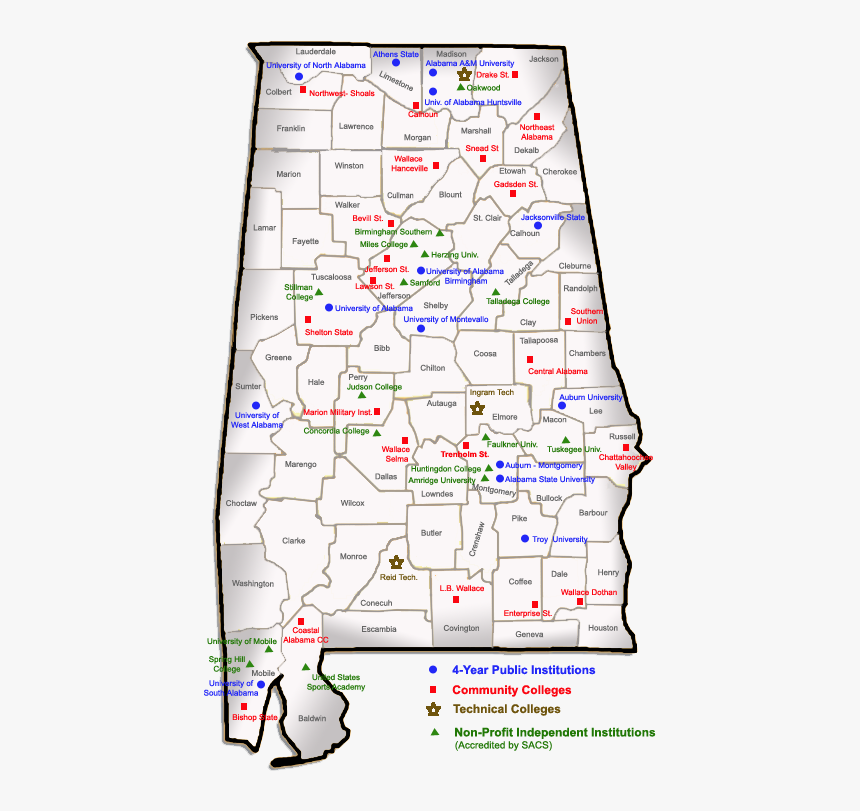
\includegraphics[scale=.4]{Figures/Figure A.1.png}
    \caption[Colleges and Universities in Alabama]{Colleges and Universities in Alabama}
    \label{fig a.1}
\end{figure}


 %This inserts your Appendix file(s). To edit this page, open the Appendix A.tex file. You will need to create a new .tex file for each appendix you want to include.



\end{document}
